\documentclass[tikz,border=8pt]{standalone}
\usepackage[T1]{fontenc}
\usepackage{lmodern}
\renewcommand{\familydefault}{\sfdefault}
\usetikzlibrary{positioning,arrows.meta,fit,backgrounds,calc}

\tikzset{
  box/.style={draw, rounded corners=2pt, align=center, font=\small\sffamily,
    fill=white, inner sep=4pt, minimum height=7mm},
  wide/.style={box, text width=110mm},
  pipe/.style={box, text width=78mm},
  frame/.style={draw, rounded corners=4pt, fill=black!4, inner sep=11pt},
  ftitle/.style={font=\small\sffamily\bfseries, anchor=north west, inner sep=1pt},
  arrow/.style={-{Latex[length=2mm,width=1.3mm]}, semithick},
  lbl/.style={font=\scriptsize\sffamily, fill=white, inner sep=1pt, align=center}
}

\begin{document}
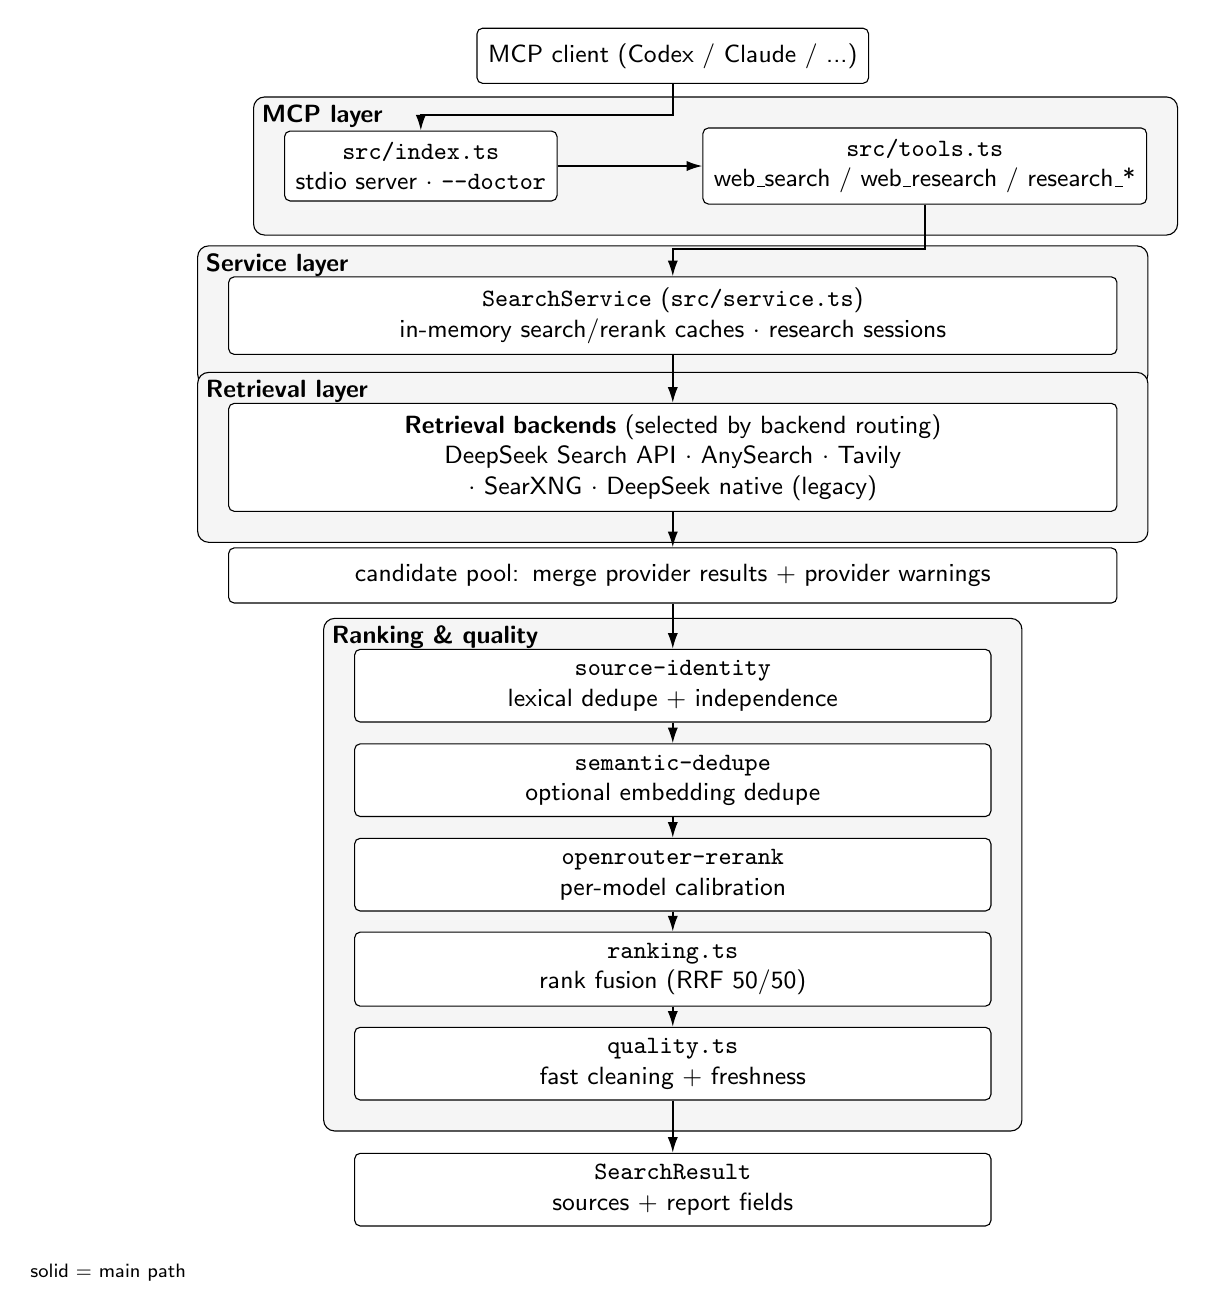
\begin{tikzpicture}
\node[box] (client) at (0,11.9) {MCP client (Codex / Claude / ...)};
\node[box] (idx) at (-3.2,10.5) {\texttt{src/index.ts}\\stdio server $\cdot$ \texttt{--doctor}};
\node[box] (tools) at (3.2,10.5) {\texttt{src/tools.ts}\\web\_search / web\_research / research\_*};
\draw[arrow] (idx) -- (tools);
\draw[arrow] (client.south) -- (0,11.15) -- (-3.2,11.15) -- (idx.north);

\node[wide] (svc) at (0,8.6) {\texttt{SearchService} (\texttt{src/service.ts})\\in-memory search/rerank caches $\cdot$ research sessions};
\draw[arrow] (tools.south) -- (3.2,9.45) -- (0,9.45) -- (svc.north);

\node[wide] (backend) at (0,6.8) {\textbf{Retrieval backends} (selected by backend routing)\\DeepSeek Search API $\cdot$ AnySearch $\cdot$ Tavily $\cdot$ SearXNG $\cdot$ DeepSeek native (legacy)};
\draw[arrow] (svc.south) -- (backend.north);

\node[wide] (pool) at (0,5.3) {candidate pool: merge provider results + provider warnings};
\draw[arrow] (backend.south) -- (pool.north);

\node[pipe] (ident) at (0,3.9) {\texttt{source-identity}\\lexical dedupe + independence};
\node[pipe] (sem) at (0,2.7) {\texttt{semantic-dedupe}\\optional embedding dedupe};
\node[pipe] (rer) at (0,1.5) {\texttt{openrouter-rerank}\\per-model calibration};
\node[pipe] (fuse) at (0,0.3) {\texttt{ranking.ts}\\rank fusion (RRF 50/50)};
\node[pipe] (qual) at (0,-0.9) {\texttt{quality.ts}\\fast cleaning + freshness};
\draw[arrow] (pool.south) -- (ident.north);
\draw[arrow] (ident) -- (sem);
\draw[arrow] (sem) -- (rer);
\draw[arrow] (rer) -- (fuse);
\draw[arrow] (fuse) -- (qual);

\node[pipe] (result) at (0,-2.5) {\texttt{SearchResult}\\sources + report fields};
\draw[arrow] (qual) -- (result);

\begin{scope}[on background layer]
  \node[frame, fit=(idx)(tools)] (f1) {};
  \node[frame, fit=(svc)] (f2) {};
  \node[frame, fit=(backend)] (f3) {};
  \node[frame, fit=(ident)(qual)] (f4) {};
\end{scope}
\node[ftitle] at ([xshift=2pt,yshift=-2pt]f1.north west) {MCP layer};
\node[ftitle] at ([xshift=2pt,yshift=-2pt]f2.north west) {Service layer};
\node[ftitle] at ([xshift=2pt,yshift=-2pt]f3.north west) {Retrieval layer};
\node[ftitle] at ([xshift=2pt,yshift=-2pt]f4.north west) {Ranking \& quality};

\node[lbl, anchor=north west, fill=none] at (-8.2,-3.4) {solid = main path};
\end{tikzpicture}
\end{document}
